
%=======================================================================
\chapter{IOMMU Support for MSIs to Virtual Machines}
\label{ch:IOMMU}

\textbf{%
Warning!
This chapter is only a draft, and might change significantly before
being ratified as standard by the {\RISCV} International Association.%
}
\bigskip

The existence of an \mbox{IOMMU} in a system makes it possible for a guest
operating system, running in a virtual machine, to be given direct
control of an I/O device with only minimal hypervisor intervention.
A guest OS with direct control of a device will program the device with
guest physical addresses, because that is all the OS knows.
When the device then performs memory accesses using those addresses, an
\mbox{IOMMU} is responsible for translating those guest physical addresses
into machine physical addresses, referencing address-translation data
structures supplied by the hypervisor.

To handle MSIs from a device controlled by a guest OS, an \mbox{IOMMU} must
be able to redirect those MSIs to a guest interrupt file in an IMSIC.
Systems that do not have IMSICs with guest interrupt files do not need
to implement the facilities described in this chapter.

Because MSIs from devices are simply memory writes, they would
naturally be subject to the same address translation that an \mbox{IOMMU}
applies to other memory writes.
However, the Advanced Interrupt Architecture requires that \mbox{IOMMU}s
treat MSIs directed to virtual machines specially, in part to
simplify software, and in part to allow optional support for
\emph{memory-resident interrupt files}.

This chapter is concerned only with how an \mbox{IOMMU} recognizes and
processes MSIs directed to virtual machines.
Most other functions and details of an \mbox{IOMMU} are beyond the scope of
this standard, and must be specified elsewhere.

If a single physical I/O device can be subdivided for multiple masters,
each sub-device is referred to here as one device.

%-----------------------------------------------------------------------
\section{Device contexts at an IOMMU}
\label{sec:IOMMU-deviceContexts}

The following assumptions are made about the \mbox{IOMMU}s in a system:
\begin{itemize}

\item
For each I/O device connected to the system through an \mbox{IOMMU},
software can configure at the \mbox{IOMMU} a \emph{device context}, which
associates with the device a specific virtual address space and any
other per-device parameters the \mbox{IOMMU} may support.
By giving devices each their own separate device context at an \mbox{IOMMU},
each device can be individually configured for a different software
master, usually a guest OS or the main (host) OS.
On every memory access made from a device, hardware indicates to
the \mbox{IOMMU} the originating device by some form of unique device
identifier, which the \mbox{IOMMU} uses to locate the appropriate device
context within data structures supplied by software.
For PCI, for example, the originating device may be identified by the
unique triple of PCI bus number, device number, and function number.

\item
An \mbox{IOMMU} optionally translates the addresses of a device's memory
accesses using address-translation data structures---typically page
tables---specified by software via the corresponding device context.
The smallest granularity of address translation implemented by all
\mbox{IOMMU}s is not larger than a \mbox{4-KiB} page, matching that of
standard {\RISCV} address-translation page tables.
(An \mbox{IOMMU} may in fact employ page tables in the same format as the
page-based address translation defined by the {\RISCV} Privileged
Architecture, but this is not required.)

\end{itemize}

The Advanced Interrupt Architecture adds to device contexts these
fields, as needed:
\begin{itemize}

\item
an \emph{MSI address mask} and \emph{address pattern}, used together to
recognize certain memory writes from the device as being MSIs; and

\item
the real physical address of an \emph{MSI page table} for controlling
the translation and/or conversion of MSIs from the device.

\end{itemize}

The MSI address mask and address pattern are each unsigned integers
with the same width as guest physical page numbers, i.e., 12~bits
narrower than the maximum supported width of a guest physical address.
Their use is explained in Section~\ref{sec:IOMMU-identIncomingMSIs},
``Identification of incoming MSIs for a virtual machine.''

A device context's MSI page table is separate from the usual
address-translation data structures used to translate other memory
accesses from the same device.
The form and function of MSI page tables are the subject of most of the
rest of this chapter.

\begin{commentary}
A device context is given an independent page table for MSIs for two
reasons:

First, hypervisors running under Linux or a similar OS can benefit from
separate control of MSI translations to help simplify the case when
virtual harts are migrated from one physical hart to another.
As noted in Section~\ref{sec:virtHartMigration}, when a virtual
hart's interrupt files are mapped to guest interrupt files in the
real machine, migration of the virtual hart causes the physical guest
interrupt files underlying those virtual interrupt files to change.
However, because on other systems (not {\RISCV}) the migration
of a virtual hart does not affect the mapping from guest physical
addresses to real physical addresses, the internal functions of Linux
that perform this migration are not set up to modify an \mbox{IOMMU}'s
address-translation tables to adjust for the changing physical
locations of {\RISCV} virtual interrupt files.
Giving a hypervisor control of a separate MSI translation table at an
\mbox{IOMMU} bypasses this limitation.
The MSI page table can be modified at will by the hypervisor and/or
by the subsystem that manages interrupts without coordinating with the
many other OS components concerned with regular address translation.

Second, specifying a separate MSI page table facilitates the use of
\emph{memory-resident interrupt files} (MRIFs), which are introduced in
Section~\ref{sec:IOMMU-MRIFs}.
A dedicated MSI page table can easily support a special table
entry format for MRIFs (Section~\ref{sec:IOMMU-MSIPTE-MRIF}) that
would be entirely foreign and difficult to retrofit to any other
address-translation data structures.
\end{commentary}

%-----------------------------------------------------------------------
\section{Translation of addresses for MSIs from devices}

To support the delivery of MSIs from I/O devices directly to {\RISCV}
virtual machines without hypervisor intervention, an \mbox{IOMMU} must be
able to translate the guest physical address of an MSI to the real
physical address of an IMSIC's guest interrupt file in the machine, as
illustrated in Figure~\ref{fig:IOMMU-guestIntrFiles}.
This address translation is controlled by the MSI page table configured
in the appropriate device context at the \mbox{IOMMU}.
Because every interrupt file, real or virtual, occupies a naturally
aligned \mbox{4-KiB} page of address space, the required address
translation is from a virtual (guest) page address to a physical page
address, the same as supported by regular {\RISCV} page-based address
translation.

\begin{figure}[th]
\centerline{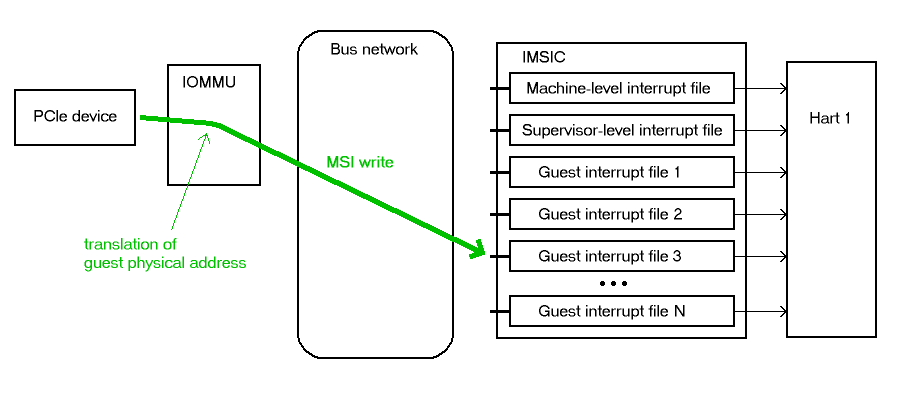
\includegraphics[scale=0.55]{IOMMU-guestIntrFiles.png}}
\caption{%
Translation of a device-sourced MSI that a guest OS intended to go to
a (virtual) IMSIC interrupt file in the OS's virtual machine.
Referencing an MSI page table supplied by the controlling hypervisor,
the \mbox{IOMMU} redirects the MSI to a guest interrupt file of the real
machine.%
}
\label{fig:IOMMU-guestIntrFiles}
\end{figure}

Memory writes from a device are recognized as MSIs by the destination
address of the write.
If an \mbox{IOMMU} determines that a \mbox{32-bit} write is to the location
of a (virtual) interrupt file in the relevant virtual machine, the
write is considered an MSI within the VM, else not.
The exact formula for recognizing MSIs is documented in
Section~\ref{sec:IOMMU-identIncomingMSIs}.

\begin{commentary}
Although the translation of MSIs is controlled by its own separate page
table, the fact that MSI translations are at the same page granularity
as regular {\RISCV} address translations implies that an address
translation cache within an \mbox{IOMMU} requires little modification to
also cache MSI translations.
Only on a translation cache miss does the \mbox{IOMMU} need to treat MSIs
significantly differently than other memory accesses from the same
device, to choose the correct translation table and to access and
interpret the table properly.
\end{commentary}

%-----------------------------------------------------------------------
\section{Memory-resident interrupt files}
\label{sec:IOMMU-MRIFs}

An \mbox{IOMMU} may optionally support memory-resident interrupt files
(MRIFs).
If implemented, the use of memory-resident interrupt files can greatly
increase the number of virtual harts that can be given direct control
of one or more physical devices in a system, assuming the rest of the
system can still handle the added load.

Without memory-resident interrupt files, the number of virtual {\RISCV}
harts that can directly receive MSIs from devices is limited by the
total number of guest interrupt files implemented by all IMSICs in the
system, because all MSIs to {\RISCV} harts must go through IMSICs.
For a single {\RISCV} hart, the number of guest interrupt files is the
\emph{GEILEN} parameter defined by the Privileged Architecture, which
can be at most 31 for RV32 and 63 for RV64.

With the use of memory-resident interrupt files, on the other hand,
the total number of virtual {\RISCV} harts able to receive device MSIs
is almost unbounded, constrained only by the amount of real physical
memory and the additional processing time needed to handle them.
As its name implies, a memory-resident interrupt file is located in
memory instead of within an IMSIC.
Figure~\ref{fig:IOMMU-MRIF} depicts how an \mbox{IOMMU} can record an
incoming MSI in an MRIF.
When properly configured by a hypervisor, an \mbox{IOMMU} recognizes certain
incoming MSIs as intended for a specific virtual interrupt file, and
records each such MSI by setting an interrupt-pending bit stored within
the MRIF data structure in ordinary memory.
After each MSI is recorded in an MRIF, the \mbox{IOMMU} also sends a
\emph{notice MSI} to the hypervisor to inform it that the MRIF contents
may have changed.

\begin{figure}[th]
\centerline{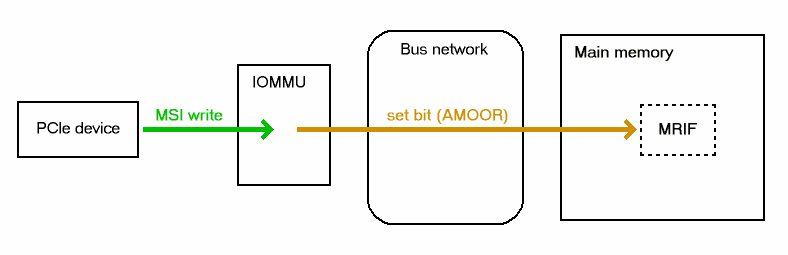
\includegraphics[scale=0.55]{IOMMU-MRIF.png}}
\caption{%
Recording an incoming MSI into a memory-resident interrupt file
(MRIF) instead of sending it to a guest interrupt file as in
Figure~\ref{fig:IOMMU-guestIntrFiles}.%
}
\label{fig:IOMMU-MRIF}
\end{figure}

While a memory-resident interrupt file provides a place to record MSIs,
it cannot interrupt a hart directly the way an IMSIC's guest interrupt
files can.
The notice MSIs that hypervisors receive only indicate that a virtual
hart \emph{might} need interrupting;
a hypervisor is responsible for examining the MRIF contents each time
to determine whether actually to interrupt the virtual hart.
Furthermore, whereas an IMSIC's guest interrupt file can directly
act as a supervisor-level interrupt file for a virtual hart, keeping
a virtual hart's interrupt file in an MRIF while the virtual hart
executes requires that the hypervisor emulate a supervisor-level
interrupt file for the virtual hart, hiding the underlying MRIF.
Depending on how often the virtual hart touches its interrupt file
and the implementation's level of support for MRIFs, the cost of this
emulation may be significant.

Consequently, MRIFs are expected most often to be used for virtual
harts that are more-or-less ``swapped out'' of a physical hart due to
being idle, or nearly so.
When a hypervisor determines that an MSI that landed in an MRIF should
wake up a particular virtual hart that was idle, the virtual hart can
be assigned a guest interrupt file in an IMSIC and its interrupt file
moved from the MRIF into this guest interrupt file before the virtual
hart is resumed.
The process of allocating a guest interrupt file for the newly wakened
virtual hart may of course force the interrupt file of another virtual
hart to be evicted to its own MRIF.

\begin{commentary}
Not all systems need to accommodate large numbers of idle virtual harts.
Many batch-processing servers, for example, strive to keep all virtual
worker threads as busy as possible from start to finish, throttled only
by I/O delays and limits on processing resources.
In such environments, support for MRIFs may not be useful, so long as
parameter GEILEN is not too small.
\end{commentary}

An \mbox{IOMMU} can have one of these three levels of support for
memory-resident interrupt files:
\begin{tightList}
\item no memory-resident interrupt files;
\item memory-resident interrupt files without atomic update; or
\item memory-resident interrupt files with atomic update.
\end{tightList}

Memory-resident interrupt files are most efficient when the memory
system supports logical atomic memory operations (AMOs) corresponding
to {\RISCV} instructions AMOAND and AMOOR, for memory accesses made
both from harts and from the \mbox{IOMMU}.
The AMOAND and AMOOR operations are required for \emph{atomic update}
of a memory-resident interrupt file.
A reduced level of support is possible without AMOs, relying solely on
basic memory reads and writes.

%- - - - - - - - - - - - - - - - - - - - - - - - - - - - - - - - - - - -
\subsection{Format of a memory-resident interrupt file}
\label{sec:IOMMU-MRIFFormat}

A memory-resident interrupt file occupies 512 bytes of memory,
naturally aligned to a \mbox{512-byte} address boundary.
The 512 bytes are organized as an array of 32 pairs of \mbox{64-bit}
doublewords, 64 doublewords in all.
Each doubleword is in little-endian byte order (even for systems where
all harts are big-endian-only).

\begin{commentary}
Big-endian-configured harts that make use of MRIFs are expected to
implement the REV8 byte-reversal instruction defined by
standard {\RISCV} extension Zbb, or pay the cost of endianness
conversion using a sequence of instructions.
\end{commentary}

The pairs of doublewords contain the interrupt-pending and
interrupt-enable bits for external interrupt identities 1--2047, in
this arrangement:
\begin{displayLinesTable}[c@{\quad}l@{\qquad}l]
offset    & \ size  & contents \\
\noalign{\medskip}
\z{0x000} & 8 bytes & interrupt-pending bits for (minor) identities 1--63 \\
\z{0x008} & 8 bytes & interrupt-enable bits for identities 1--63 \\
\z{0x010} & 8 bytes & interrupt-pending bits for identities 64--127 \\
\z{0x018} & 8 bytes & interrupt-enable bits for identities 64--127 \\
\dots     &         & \ \dots \\
\z{0x1F0} & 8 bytes & interrupt-pending bits for identities 1984--2047 \\
\z{0x1F8} & 8 bytes & interrupt-enable bits for identities 1984--2047 \\
\end{displayLinesTable}
In general, the pair of doublewords at address offsets
$k\times\mbox{16}$ and ${k\times\mbox{16}+\mbox{8}}$ for integer $k$
contain the interrupt-pending and interrupt-enable bits for external
interrupt minor identities in the range $k\times\mbox{64}$ to
$k\times\mbox{64}+\mbox{63}$.
For identity~$i$ in this range, bit $(i\bmod\mbox{64})$ of the first
(even) doubleword is the interrupt-pending bit, and the same bit of the
second (odd) doubleword is the interrupt-enable bit.

\begin{commentary}
The interrupt-pending and interrupt-enable bits are stored interleaved
by doublewords within an MRIF to facilitate the possibility of an
\mbox{IOMMU} examining the relevant enable bit to determine whether to send
a notice MSI after updating a pending bit, rather than the default
behavior of always sending a notice MSI after an update without regard
for the interrupt-enable bits.
The memory arrangement matters only when MRIFs are supported without
atomic update.
\end{commentary}

Bit~0 of the first doubleword of an MRIF stores a faux
interrupt-pending bit for nonexistent interrupt~0.
If a write from an I/O device appears to be an MSI that should be
stored in an MRIF, yet the data to write (the interrupt identity) is
zero, the \mbox{IOMMU} acts as though zero were a valid interrupt identity,
setting bit~0 of the target MRIF's first doubleword and sending a
notice MSI as usual.

All MRIFs are the size to accommodate 2047 valid interrupt identities,
the maximum allowed for an IMSIC interrupt file.
If a system's actual IMSICs have interrupt files that implement
only $N$ interrupt identities, ${N < \mbox{2047}}$, then the contents
of MRIFs for identities greater than $N$ may be ignored by software.
\mbox{IOMMU}s, however, treat every MRIF as though all interrupt identities
in the range 0--2047 are valid, even as software ignores invalid
identity~0 and all identities greater than~$N$.

\begin{commentary}
There is no need to specify to an \mbox{IOMMU} a desired size~$N$ for an
MRIF smaller than 2047 valid interrupt identities.
The only use an \mbox{IOMMU} would make of this information would be to
discard any MSIs indicating an interrupt identity greater than~$N$.
If devices are properly configured by software, such errant MSIs should
not occur;
but even if they do, it is just as effective for software to ignore
spurious interrupt identities \emph{after} they have been recorded in
an MRIF as for an \mbox{IOMMU} to discard them before recording them in the
MRIF.

It is likewise unnecessary for \mbox{IOMMU}s to check for and discard MSIs
indicating an invalid interrupt identity of zero.
\end{commentary}

%- - - - - - - - - - - - - - - - - - - - - - - - - - - - - - - - - - - -
\subsection{Recording of incoming MSIs to memory-resident interrupt files}

The data component of an MSI write specifies the interrupt identity to
raise in the destination interrupt file.
(Recall Section~\ref{sec:MSIEncoding}.)
This data may be in little-endian or big-endian byte order.
If an \mbox{IOMMU} supports memory-resident interrupt files, it can store to
an MRIF MSIs of the same endianness that the machine's IMSICs accept.
All IMSIC interrupt files are required to accept MSIs in little-endian
byte order written to memory-mapped register \z{seteipnum\_le}
(Section~\ref{sec:IMSIC-memRegion}).
IMSIC interrupt files may also accept MSIs in big-endian byte order if
register \z{seteipnum\_be} is implemented alongside \z{seteipnum\_le}.

If the interrupt identity indicated by an MSI's data (when interpreted
in the correct byte order) is in the range 0--2047, an \mbox{IOMMU} stores
the MSI to an MRIF by setting to one the interrupt-pending bit in the
MRIF for that identity.
If atomic update is supported for MRIFs, the pending bit is set using
an AMOOR operation, else it is set using a non-atomic read-modify-write
sequence.
After the interrupt-pending bit is set in the MRIF, the \mbox{IOMMU} sends
the notice MSI that software has configured for the MRIF.

The exact process of storing an MSI to an MRIF is specified more
precisely in Section~\ref{sec:IOMMU-MSIPTE-MRIF}, which covers MSI page
table entries configured in \emph{MRIF mode}.

\begin{commentary}
It is an open question whether an \mbox{IOMMU} might optionally examine
the matching interrupt-enable bit within a destination MRIF to decide
whether to send a notice MSI after setting an interrupt-pending bit.
Currently, an \mbox{IOMMU} is required always to send a notice MSI after
storing an MSI to an MRIF, even when the corresponding enable bit for
the interrupt identity is zero.
\end{commentary}

%- - - - - - - - - - - - - - - - - - - - - - - - - - - - - - - - - - - -
\subsection{Use of memory-resident interrupt files with atomic update}

To make use of a memory-resident interrupt file with support for atomic
update, software must have memory locations to save an IMSIC interrupt
file's \z{eidelivery} and \z{eithreshold} registers, in addition to the
MRIF structure itself from Section~\ref{sec:IOMMU-MRIFFormat}.

Moving a virtual hart's interrupt file from an IMSIC into an MRIF
involves these steps:
\begin{enumerate}

\item
Prepare the MRIF by zeroing all of its interrupt-pending bits (the even
doublewords) and by copying the IMSIC interrupt file's \z{eie} array to
the MRIF's interrupt-enable bits (the odd doublewords).

\item
At the IMSIC interrupt file, save to memory the existing values of
registers \z{eidelivery} and \z{eithreshold}, and set \z{eidelivery}
=~0.

\item
Modify all relevant translation tables at \mbox{IOMMU}s so that MSIs for
this virtual interrupt file are now stored in the MRIF.
If necessary, synchronize with all \mbox{IOMMU}s to ensure that no straggler
MSIs will arrive at the old IMSIC interrupt file after this step.

\item
Logically OR the contents of the IMSIC interrupt file's \z{eip} array
into the interrupt-pending bits of the MRIF, using AMOOR operations.

\end{enumerate}
Once this sequence is complete, the IMSIC interrupt file is no longer
in use.

Each time a notice MSI arrives indicating that an MSI has been
stored in the MRIF, the controlling hypervisor should scan the MRIF's
interrupt-pending and interrupt-enable bits to determine if any enabled
interrupt is now both pending and enabled and thus should interrupt the
virtual hart.

With atomic update of MRIFs, a virtual hart may continue executing
with its interrupt file contained in an MRIF, so long as the hypervisor
emulates for the virtual hart a proper IMSIC interrupt file to hide the
underlying MRIF.
Hypervisor software can safely set and clear the interrupt-pending and
interrupt-enable bits of the MRIF using AMOOR and AMOAND operations,
even as an \mbox{IOMMU} may be storing incoming MSIs into the same MRIF.

\begin{commentary}
If an \mbox{IOMMU} is ever configured to examine an MRIF's interrupt-enable
bits to decide whether to send notice MSIs, then modifying those enable
bits will generally require coordination with the \mbox{IOMMU}.
But so long as \mbox{IOMMU}s ignore the interrupt-enable bits as is
currently assumed, the bits can be changed by software without risk.
\end{commentary}

To move the same interrupt file from the MRIF back to an IMSIC:
\begin{enumerate}

\item
At the new IMSIC interrupt file, set \z{eidelivery} =~0, and zero the
\z{eip} array.

\item
Modify all relevant translation tables at \mbox{IOMMU}s so that MSIs for
this virtual interrupt file are now sent to the IMSIC interrupt file.
If necessary, synchronize with all \mbox{IOMMU}s to ensure that no straggler
MSIs will be stored in the MRIF after this step.

\item
Logically OR the interrupt-pending bits from the MRIF into the IMSIC
interrupt file, using instruction CSRS to write to the \z{eip} array.
Also, copy the interrupt-enable bits from the MRIF to the IMSIC
interrupt file's \z{eie} array.

\item
At the IMSIC interrupt file, load registers \z{eithreshold} and
\z{eidelivery} with the values that were earlier saved.

\end{enumerate}

%- - - - - - - - - - - - - - - - - - - - - - - - - - - - - - - - - - - -
\subsection{Use of memory-resident interrupt files without atomic update}

Without support for atomic update, the use of memory-resident interrupt
files is similar to the atomic-update case of the previous subsection,
but with some added complexities.

First, if the I/O devices that a virtual hart controls are behind
multiple \mbox{IOMMUs}, then multiple MRIF structures are needed, one per
\mbox{IOMMU}, not just a single MRIF structure.
Furthermore, in addition to locations for storing \z{eidelivery} and
\z{eithreshold}, software needs a place for a complete copy of the
interrupt file's implemented \z{eip} array, apart from the MRIFs.
While a virtual interrupt file is in memory, its interrupt-pending bits
will be split across all the MRIFs and the saved \z{eip} array.
The interrupt-enable bits will exist only in the MRIFs.

To move a virtual hart's interrupt file from an IMSIC into memory, with
one MRIF per \mbox{IOMMU}:
\begin{enumerate}

\item
Prepare all MRIFs by zeroing their interrupt-pending bits (the even
doublewords) and by copying the IMSIC interrupt file's \z{eie} array to
the MRIFs' interrupt-enable bits (the odd doublewords).

\item
At the IMSIC interrupt file, save to memory the existing values of
registers \z{eidelivery} and \z{eithreshold}, and set \z{eidelivery}
=~0.

\item
At each \mbox{IOMMU}, modify all relevant translation tables so that MSIs
for this virtual interrupt file are now stored in the individual MRIF
matched to the \mbox{IOMMU}.
If necessary, synchronize with all \mbox{IOMMU}s to ensure that no straggler
MSIs will arrive at the old IMSIC interrupt file after this step.

\item
Dump the IMSIC interrupt file's \z{eip} array to its separate location
outside the MRIFs.

\end{enumerate}
Once this sequence is complete, the IMSIC interrupt file is no longer
in use.

While a virtual hart's interrupt file remains in memory, an interrupt
identity's true pending bit is the logical OR of its bit in all MRIFs
and its bit in the saved \z{eip} array.
All pending bits in the MRIFs start as zeros, but interrupts may become
pending there as MSIs for this virtual hart arrive at \mbox{IOMMU}s and are
stored in the corresponding MRIFs.

Without atomic update of MRIFs, an interrupt-pending bit is not easily
cleared in an MRIF.
(Clearing a single pending bit in one MRIF requires that a new MRIF be
allocated and initialized and the corresponding \mbox{IOMMU} reconfigured to
store MSIs into the new MRIF.)
For this reason, it may or may not be practical to have a virtual hart
execute while keeping one of its interrupt files in memory.
When an MRIF records an interrupt that should wake a virtual hart, the
simplest strategy is to always move the interrupt file back into an
IMSIC's guest interrupt file before resuming execution of the virtual
hart.

To transfer an interrupt file from memory back to an IMSIC:
\begin{enumerate}

\item
At the new IMSIC interrupt file, set \z{eidelivery} =~0, and zero the
\z{eip} array.

\item
Modify all relevant translation tables at \mbox{IOMMU}s so that MSIs for
this virtual interrupt file are now sent to the IMSIC interrupt file.
If necessary, synchronize with all \mbox{IOMMU}s to ensure that no straggler
MSIs will be stored in MRIFs after this step.

\item
Merge by bitwise logical OR the interrupt-pending bits of all MRIFs and
the saved \z{eip} array, and logically OR these merged bits into the
IMSIC interrupt file, using instruction CSRS to write to the \z{eip}
array.
Also, copy the interrupt-enable bits from one of the MRIFs to the IMSIC
interrupt file's \z{eie} array.

\item
At the IMSIC interrupt file, load registers \z{eithreshold} and
\z{eidelivery} with the values that were earlier saved.

\end{enumerate}

%- - - - - - - - - - - - - - - - - - - - - - - - - - - - - - - - - - - -
\subsection{Allocation of guest interrupt files for receiving notice MSIs}

The processing a hypervisor does in response to notice MSIs can be
minimized by assigning a separate interrupt identity for each MRIF, so
the identity encoded in a notice MSI always indicates which one MRIF
may have changed.
However, if there are very many MRIFs (potentially in the thousands),
a hypervisor may run short of interrupt identities within the
supervisor-level interrupt files available in IMSICs.
In that case, the hypervisor can increase its supply of interrupt
identities by allocating one or more of the IMSICs' guest interrupt
files to itself for the purpose of receiving notice MSIs.

\begin{commentary}
Although guest interrupt files exist primarily to act as
supervisor-level interrupt files for virtual harts, the IMSIC hardware
does not police exactly how they are used by software.
\end{commentary}

%-----------------------------------------------------------------------
\section{Identification of incoming MSIs for a virtual machine}
\label{sec:IOMMU-identIncomingMSIs}

When an I/O device is configured directly by a guest operating system,
MSIs from the device are expected to be targeted to virtual IMSICs
within the guest OS's virtual machine, using guest physical addresses
that are inappropriate and unsafe for the real machine.
An \mbox{IOMMU} must recognize certain incoming writes from such devices as
MSIs and convert them as needed for the real machine.
(Recall Figure~\ref{fig:IOMMU-guestIntrFiles}.)

MSIs originating from a single device that require conversion are
expected to have been configured at the device by a single guest OS
running within one {\RISCV} virtual machine.
Assuming the VM itself conforms to the Advanced Interrupt Architecture,
MSIs are sent to virtual harts within the VM by writing to the
memory-mapped registers of the interrupt files of virtual IMSICs.
Each of these virtual interrupt files occupies a separate \mbox{4-KiB}
page in the VM's guest physical address space, the same as real
interrupt files do in a real machine's physical address space.
A write to a guest physical address can thus be recognized as an MSI to
a virtual hart if the write is to a page occupied by an interrupt file
of a virtual IMSIC within the VM.

The MSI address mask and address pattern specified in a device context
(Section~\ref{sec:IOMMU-deviceContexts}) are used to identify the
\mbox{4-KiB} pages of virtual interrupt files in the guest physical
address space of the relevant VM.
An incoming \mbox{32-bit} write made by a device is recognized as an
MSI write to a virtual interrupt file if the destination guest physical
page matches the supplied address pattern in all bit positions that are
zeros in the supplied address mask.
In detail, a write to guest physical address~$A$ is recognized as an
MSI to a virtual interrupt file if
$$
\bigl(\mbox{($A$\,\z{>>}\,12) \z{\&} $\sim$address mask}\bigr)
  = (\mbox{address pattern \z{\&} $\sim$address mask})
$$
where \mbox{\z{>>}\,12} represents shifting right by 12~bits,
an ampersand (\z{\&}) represents bitwise logical AND, and
``$\sim$address mask'' is the bitwise logical complement of the address
mask.

When a write is identified as an MSI from a device, an
\emph{interrupt file number} is extracted from the original guest
physical address as
\begin{displayLinesTable}
interrupt file number = extract($A$\,\z{>>}\,12, address mask) \\
\end{displayLinesTable}
The extract function here is the same generic bit extract performed
by {\RISCV} instruction BEXT, defined by the ``Bitmanip'' extension
(B~extension).
The bit extract function extract($x$,~$y$) discards all bits from
$x$ whose matching bits in the same positions in the mask~$y$ are
zeros, and packs the remaining bits from $x$ contiguously at the
least-significant end of the result, keeping the same bit order as $x$
and filling any other bits at the most-significant end of the result
with zeros.
For example, if the bits of $x$ and $y$ are
\begin{displayLinesTable}[r@{ }c@{ }c@{ }c@{ }c@{ }c@{ }c@{ }c@{ }c]
$x$ = & a & b & c & d & e & f & g & h \\
$y$ = & 1 & 0 & 1 & 0 & 0 & 1 & 1 & 0 \\
\end{displayLinesTable}
then the value of extract($x$,~$y$) has bits 0~0~0~0~a~c~f~g.

%-----------------------------------------------------------------------
\section{MSI page tables}

Whenever an \mbox{IOMMU} recognizes an incoming write from a device as
an MSI by the method specified in the previous section, the MSI is
translated or converted by consulting the MSI page table configured for
the device, instead of using the regular translation data structures
that apply to all other memory accesses from the same device.

Only naturally aligned \mbox{32-bit} writes from a device are possible
MSIs.
For other forms of memory accesses by a device (such as reads, writes
of other sizes, or misaligned writes), the regular translation data
structures are always applied, even if the address matches that of a
proper MSI.

An MSI page table is a flat array of MSI page table entries (MSI PTEs),
each 16~bytes.
MSI page tables have no multi-level hierarchy like regular {\RISCV}
page tables do.
Rather, every MSI PTE is a leaf entry specifying the translation or
conversion of writes made to a particular \mbox{4-KiB} guest physical
page that a virtual interrupt file occupies (or may occupy) in the
relevant virtual machine.
To select an individual MSI PTE from an MSI page table, the PTE array
is indexed by the interrupt file number extracted from the destination
guest physical address of the incoming MSI write by the formula of the
previous section.
Each MSI PTE may specify either the address of a real guest interrupt
file that substitutes for the targeted virtual interrupt file (as in
Figure~\ref{fig:IOMMU-guestIntrFiles}), or a memory-resident interrupt
file in which to store incoming MSIs for the virtual interrupt file
(as in Figure~\ref{fig:IOMMU-MRIF}).

The number of entries in an MSI page table is always a power of two,
specifically $\mbox{2}^{k}$ where $k$ is the number of bits that are
ones in the MSI address mask used to extract the interrupt file number
from the destination guest physical address.
If an MSI page table has 256 or fewer entries, the start of the table
is always aligned to a \mbox{4-KiB} page address in real physical
memory.
If an MSI page table has ${\mbox{2}^{k} > \mbox{256}}$
entries, the table must be naturally aligned to a
$\mbox{2}^{k}\times \mbox{16-byte}$ address boundary.
If an MSI page table is not aligned as required, all entries in the
table appear to an \mbox{IOMMU} as {\unspecified}, and any address an
\mbox{IOMMU} may compute and use for reading an individual MSI PTE from the
table is also {\unspecified}.

Every \mbox{16-byte} MSI PTE is interpreted as two \mbox{64-bit}
doublewords.
If an \mbox{IOMMU} also references standard {\RISCV} page tables, defined by
the {\RISCV} Privileged Architecture, for regular address translation,
then the byte order for each of the two doublewords in memory,
little-endian or big-endian, should be the same as the endianness
of the regular {\RISCV} page tables configured for the same device
context.
Otherwise, the endianness of the doublewords of an MSI PTE is
implementation-defined.

Bit~0 of the first doubleword of an MSI PTE is field~V (Valid).
When V~=~0, the PTE is invalid, and all other bits of both doublewords
are ignored by an \mbox{IOMMU}, making them free for software to use.

If V~=~1, bit~63 of the first doubleword is field~C (Custom),
designated for custom use.
If an MSI PTE has V~=~1 and C~=~1, interpretation of the rest of the
PTE is implementation-defined.

If V~=~1 and the custom-use bit C~=~0, then bit~2 of the first
doubleword is field~W (Write-through).
If W~=~1, the MSI PTE specifies \emph{write-through mode} for incoming
MSIs, and if W~=~0, it specifies \emph{MRIF mode}.
The interpretation of an MSI PTE for each of these two modes is
detailed further in the next two subsections.

%- - - - - - - - - - - - - - - - - - - - - - - - - - - - - - - - - - - -
\subsection{MSI PTE, write-through mode}

When an MSI PTE has fields V~=~1, C~=~0, and W~=~1
(write-through mode), the PTE's complete format is:\nopagebreak
\begin{displayLinesTable}[l@{\quad}l@{\quad}l]
First doubleword:  & bit 63     & C, = 0 \\
                   & bits 53:10 & PPN \\
                   & bit 2      & W, = 1 \\
                   & bit 0      & V, = 1 \\
\noalign{\medskip}
Second doubleword: & ignored \\
\end{displayLinesTable}
All other bits of the first doubleword are reserved and must be set to
zeros by software.
The second doubleword is ignored by an \mbox{IOMMU} so is free for software
to use.

An incoming MSI write is translated by replacing the write's original
address bits 12 and above (the guest physical page number) with field
PPN (Physical Page Number) from the PTE, while retaining the original
address bits 11:0 (the page offset).
This translated address is either zero-extended or clipped at the upper
end as needed to make it the width of a real physical address for the
machine.
The original memory write from the device is then passed onward to the
memory system with the new address.

An MSI PTE in write-through mode allows a hypervisor to route an
MSI intended for a virtual interrupt file to go instead to a guest
interrupt file of a real IMSIC in the machine.

\begin{commentary}
An \mbox{IOMMU} that also employs standard {\RISCV} page tables for regular
address translation can maximize the overlap between the handling of
MSI PTEs and regular {\RISCV} leaf PTEs as follows:

For RV64, the first doubleword of an MSI PTE in write-through mode
has the same encoding as a regular {\RISCV} leaf PTE for Sv39, Sv48,
Sv39x4, or Sv48x4 page-based address translation, with PTE fields D, A,
G, U, X, and R all zeros and W~=~1.
Hence, the MSI PTE's first doubleword appears the same as a regular
PTE that grants write permission (W~=~1) but not read or execute
permissions (X~= R =~0).
This same-encoded regular PTE would translate an MSI write the same as
the actual MSI PTE, except that what would be the PTE's accessed (A),
dirty (D), and user (U) bits are all zeros.
An \mbox{IOMMU} needs to treat only these three bits differently for an MSI
PTE versus a regular RV64 leaf PTE.

The address computation used to select a PTE from a regular {\RISCV}
page table must be modified to select an MSI PTE's first doubleword
from an MSI page table.
However, the extraction of an interrupt file number from a guest
physical address to obtain the index for accessing the MSI page table
already creates an unavoidable difference in PTE addressing.

For RV32, the lower \mbox{32-bit} word of an MSI PTE's first doubleword
has the same format as a leaf PTE for Sv32 or Sv32x4 page-based address
translation, except again for what would be PTE bits A, D, and~U, which
must be treated differently.
\end{commentary}

%- - - - - - - - - - - - - - - - - - - - - - - - - - - - - - - - - - - -
\subsection{MSI PTE, MRIF mode}
\label{sec:IOMMU-MSIPTE-MRIF}

If memory-resident interrupt files are supported and an MSI PTE has
fields V~=~1, C~=~0, and W~=~0 (MRIF mode), the PTE's complete format
is:\nopagebreak
\begin{displayLinesTable}[l@{\quad}l@{\quad}l]
First doubleword:  & bit 63     & C, = 0 \\
                   & bits 53:7  & MRIF Address[55:9] \\
                   & bit 2      & W, = 0 \\
                   & bit 0      & V, = 1 \\
\noalign{\medskip}
Second doubleword: & bit 60     & NID[10] \\
                   & bits 53:10 & NPPN \\
                   & bits 9:0   & NID[9:0] \\
\end{displayLinesTable}
All other PTE bits are reserved and must be set to zeros by software.

The PTE's MRIF Address field provides bits 55:9 of the physical address
of a memory-resident interrupt file in which to store incoming MSIs,
referred to as the \emph{destination MRIF}.
As every memory-resident interrupt file is naturally aligned to a
\mbox{512-byte} address boundary, bits 8:0 of the destination MRIF's
address must be zero and are not specified in the PTE.

Field NPPN (Notice Physical Page Number) and the two NID
(Notice Identifier) fields together specify a destination and value for
a \emph{notice MSI} that is sent after each time the destination MRIF
is updated as a result of consulting this PTE to store an incoming MSI.

\begin{commentary}
Typically, NPPN will be the page address of an IMSIC's interrupt file
in the real machine, and NID will be the interrupt identity to make
pending in that interrupt file to indicate that the destination MRIF
may have changed.
However, NPPN is not required to be a valid interrupt file address, and
an \mbox{IOMMU} must not attempt to restrict it to only such addresses.
Any page address must be accepted for NPPN.
\end{commentary}

When the IMSIC interrupt files in the system implement memory-mapped
register \z{seteipnum\_be} for receiving MSIs in big-endian byte order
(Section~\ref{sec:IMSIC-memRegion}), then an \mbox{IOMMU} must be able to
store MSIs in both little-endian and big-endian byte orders to the
destination MRIF.
If the IMSIC interrupt files in the system do not implement
register \z{seteipnum\_be}, an \mbox{IOMMU} should ordinarily store only
little-endian MSIs to the destination MRIF.
The data of an incoming MSI is assumed to be in little-endian byte
order if bit~2 of the destination address is zero, and in big-endian
byte order if bit~2 of the destination address is one.

If the incoming MSI write is to guest physical address~$A$ and its
\mbox{32-bit} data is~$D$ when interpreted in the byte order indicated
by bit~2 of $A$, then the MSI is processed by the \mbox{IOMMU} as follows:
If either $A$\z{[}11:3\z{]} or $D$\z{[}31:11\z{]} is not zero, or if
bit~2 of $A$ is one and big-endian MSIs are not supported, then the
incoming write is accepted but discarded.
Else, the original incoming write is replaced by this sequence:
\begin{enumerate}

\item
In the destination MRIF, set the interrupt-pending bit for interrupt
identity $D$ to one, using either an AMOOR operation for atomic update,
or a non-atomic read-modify-write sequence.

\item
Zero-extend the \mbox{11-bit} NID value to 32~bits, and do a
\mbox{32-bit} write of this value in little-endian byte order to the
address NPPN\,\z{<<}\,12 (i.e., physical page number NPPN, page offset
zero).

\end{enumerate}
The write of step~1 must be visible to all agents in the system before
the write of step~2 becomes visible to any agent.

\begin{commentary}
While \mbox{IOMMU}s are expected typically to cache MSI PTEs that are
configured in write-through mode (W~=~1), they might not cache PTEs
configured in MRIF mode (W~=~0).
Two reasons together justify not caching MSI PTEs in MRIF mode:
First, the information and actions required to store an MSI to an MRIF
are far different than normal address translation; and
second, by their nature, MSIs to MRIFs should occur less frequently.
Hence, an \mbox{IOMMU} might perform MRIF-mode processing solely as
an extension of cache-miss page table walks, leaving its address
translation cache oblivious to MRIF-mode MSI PTEs.
\end{commentary}

